\documentclass[aspectratio=169,11pt]{beamer}

% Sprache und Schrift (xelatex)
\usepackage{fontspec}
\usepackage[ngerman,provide=*]{babel}
\usepackage{csquotes}

% Beamer-Theme: schlicht, akademisch
\usetheme{default}
\usecolortheme{dove}
\setbeamertemplate{navigation symbols}{}
\setbeamerfont{title}{size=\Large,series=\bfseries}
\setbeamerfont{frametitle}{size=\large,series=\bfseries}
\setbeamercolor{frametitle}{fg=black}
\setbeamercolor{title}{fg=black}
\setbeamercolor{structure}{fg=black!75}
\setbeamercolor{normal text}{fg=black!90}
\setbeamertemplate{itemize item}{\textbullet}
\setbeamertemplate{itemize subitem}{\textendash}

\setbeamertemplate{footline}{%
  \leavevmode%
  \hbox{%
    \begin{beamercolorbox}[wd=.55\paperwidth,ht=2.25ex,dp=1ex,leftskip=1em]{author in head/foot}%
      \footnotesize\color{black!60}MTA -- Sitzung 2: Wie funktionieren Topic-Modelle?%
    \end{beamercolorbox}%
    \begin{beamercolorbox}[wd=.45\paperwidth,ht=2.25ex,dp=1ex,rightskip=1em,leftskip=2ex]{title in head/foot}%
      \hfill\footnotesize\color{black!60}\insertframenumber\,/\,\inserttotalframenumber%
    \end{beamercolorbox}}%
}

\usepackage{booktabs}
\usepackage{array}
\usepackage{tabularx}
\usepackage{amsmath}
\usepackage{tikz}
\usetikzlibrary{positioning,arrows.meta,calc,matrix,fit}

% ---------------------------------------------------------------
\title{Wie funktionieren Topic-Modelle?}
\subtitle{Sitzung 2 -- Mathematische Grundlagen,\\LDA, NMF und der Sprung zu BERT/LLMs}
\author{Prof.~Dr.~Christian Papilloud}
\institute{Institut für Soziologie\\Martin-Luther-Universität Halle-Wittenberg}
\date{Master Soziologie -- 2026}

\begin{document}

% ===============================================================
\begin{frame}[plain]
  \titlepage
\end{frame}

% ===============================================================
\begin{frame}{Wo wir stehen}

  In der letzten Sitzung haben wir Topic-Modelle (TM) \emph{methodologisch}
  positioniert: Sie sind \emph{quantitativ basiert}, dienen aber der
  qualitativen Forschung -- näher an Mayring als an Oevermann.

  \vfill
  Heute fragen wir: \textbf{Wie funktioniert das technisch?}

  \vfill
  Vier Blöcke:
  \begin{enumerate}
    \item[\textbf{1.}] Was ist ein \emph{topic}? Die Matrixfaktorisierung
          anhand eines kleinen Beispiels (\enquote{MLU/Sommer}).
    \item[\textbf{2.}] Vergleich mit zwei verwandten Verfahren:
          \emph{Clusteranalyse} und \emph{Faktorenanalyse}.
    \item[\textbf{3.}] Die zwei klassischen TM-Verfahren:
          \textbf{LDA} und \textbf{NMF}.
    \item[\textbf{4.}] \emph{Neue Welt:} \textbf{BERTopic} und \textbf{LLMs}.
          Was ändert sich? Warum bleibt MTA bei LDA/NMF?
  \end{enumerate}

\end{frame}

% ===============================================================
\section{1. Was ist ein topic?}

\begin{frame}{Die zentrale Intuition}

  \begin{block}{Definition (sehr informell)}
    Ein \emph{topic} ist eine \textbf{Wortliste} -- eine Gruppe von
    Wörtern, die \emph{oft gemeinsam} in Dokumenten vorkommen.
    \\[4pt]
    Wenn \enquote{Milch} und \enquote{Katze} immer wieder gemeinsam
    auftauchen, gibt es vermutlich ein topic, das beide enthält.
  \end{block}

  \vfill
  Ein Topic-Modell liefert zwei Dinge:
  \begin{itemize}
    \item \textbf{Topic-Wort-Zugehörigkeit:} Welche Wörter bilden welches
          topic? (Mit welchem Gewicht?)
    \vfill
    \item \textbf{Topic-Gewichte der Dokumente:} Welche Dokumente
          enthalten welche topics? (In welchem Anteil?)
  \end{itemize}

  \vfill
  Diese beiden Ergebnisse sind das, was wir in MTA als CSV-Dateien
  und Heatmaps wiederfinden werden.

\end{frame}

% ===============================================================
\begin{frame}{Beispiel: drei Dokumente, acht Wörter}

  Dokumente (Papilloud \& Hinneburg 2018, Abb.~2.1):
  \vfill
  \footnotesize
  \begin{tabularx}{\textwidth}{@{}p{0.10\textwidth}X@{}}
    \toprule
    \textbf{Dok.\ 1} & Die Studenten der MLU können die Teile des Campus im
                       Sommer per Fahrrad erreichen. \\
    \textbf{Dok.\ 2} & Im Sommer gehen Menschen gern schwimmen oder fahren
                       Fahrrad. \\
    \textbf{Dok.\ 3} & Die MLU bietet auf ihrem Campus den Studenten
                       kostenlos Internet an. \\
    \bottomrule
  \end{tabularx}

  \vfill
  \normalsize
  Reduziert auf \emph{Substantive}: Campus, Fahrrad, Internet, Mensch,
  Sommer, Student, Teil, MLU.

  \vfill
  Inhaltlich erkennen wir intuitiv \emph{zwei Themen}:
  \textbf{Universität} (MLU, Campus, Student, Internet)
  und \textbf{Sommer} (Sommer, Fahrrad, Mensch).

  \vfill
  Die Frage: kann ein Algorithmus diese zwei Themen \emph{ohne Vorwissen}
  finden? Die Antwort: ja, durch Matrixfaktorisierung.

\end{frame}

% ===============================================================
\begin{frame}{Schritt 1: Dokument-Wort-Matrix $A$}

  Wir bauen eine Tabelle: Zeilen = Dokumente, Spalten = Wörter.
  Eintrag = wie oft kommt das Wort im Dokument vor?

  \vfill
  \begin{center}
    \footnotesize
    \begin{tabular}{@{}l|cccccccc@{}}
      \toprule
      & Campus & Fahrrad & Internet & Mensch & Sommer & Student & Teil & MLU \\
      \midrule
      Dok.\ 1 & 1 & 1 & 0 & 0 & 1 & 1 & 1 & 1 \\
      Dok.\ 2 & 0 & 1 & 0 & 1 & 1 & 0 & 0 & 0 \\
      Dok.\ 3 & 1 & 0 & 1 & 0 & 0 & 1 & 0 & 1 \\
      \bottomrule
    \end{tabular}
  \end{center}

  \vfill
  Diese \textbf{Dokument-Wort-Matrix} $A$ ist der Input jedes
  Topic-Modells. Bei einem realen Korpus von 10\,000 Texten mit
  einem Vokabular von 5\,000 Wörtern hat sie 50 Millionen Einträge --
  meistens Nullen (\emph{sparse matrix}).

\end{frame}

% ===============================================================
\begin{frame}{Schritt 2: Faktorisierung in zwei kleinere Matrizen}

  Ein Topic-Modell zerlegt $A$ in das \emph{Produkt zweier kleinerer
  Matrizen}:
  \[
    \underbrace{A}_{\text{Dokumente}\times\text{Wörter}}
    \;\approx\;
    \underbrace{W}_{\text{Dokumente}\times K}
    \;\cdot\;
    \underbrace{H}_{K\times\text{Wörter}}
  \]
  wobei $K$ die Anzahl der topics ist (hier: $K=2$).

  \vfill
  Was bedeutet das? \\[6pt]
  -- $W$ sagt: \emph{Welches topic in welchem Dokument?} (Topic-Gewichte) \\
  -- $H$ sagt: \emph{Welche Wörter in welchem topic?} (Topic-Inhalt)

  \vfill
  Statt $3\times 8 = 24$ Werte (in $A$) brauchen wir nur
  $3\times 2 + 2\times 8 = 22$ Werte (in $W$ und $H$).
  Bei größeren Matrizen ist die Reduktion enorm -- und sie zwingt das
  Modell, die \emph{wesentlichen Strukturen} zu finden.

\end{frame}

% ===============================================================
\begin{frame}{Ergebnis im Beispiel}

  \textbf{Topic-Wort-Zugehörigkeit $H$} -- welche Wörter bilden welches topic:
  \footnotesize
  \begin{center}
    \begin{tabular}{@{}l|cccccccc@{}}
      \toprule
      & Campus & Fahrrad & Internet & Mensch & Sommer & Student & Teil & MLU \\
      \midrule
      Topic 1 (\textit{Uni}) & 1 & 0 & 1 & 0 & 0 & 1 & 1 & 1 \\
      Topic 2 (\textit{Sommer}) & 0 & 1 & 0 & 1 & 1 & 0 & 0 & 0 \\
      \bottomrule
    \end{tabular}
  \end{center}

  \normalsize
  \vfill
  \textbf{Topic-Gewichte der Dokumente $W$}:
  \footnotesize
  \begin{center}
    \begin{tabular}{@{}l|cc@{}}
      \toprule
      & Topic 1 & Topic 2 \\
      \midrule
      Dok.\ 1 & 1 & 1 \\
      Dok.\ 2 & 0 & 1 \\
      Dok.\ 3 & 1 & 0 \\
      \bottomrule
    \end{tabular}
  \end{center}

  \normalsize
  \vfill
  Dok.\ 1 enthält \emph{beide} topics. Dok.\ 2 nur Sommer. Dok.\ 3 nur Uni.

\end{frame}

% ===============================================================
\begin{frame}{Wie findet der Algorithmus diese Zerlegung?}

  Das Problem ist \emph{zirkulär}:
  \begin{itemize}
    \item Wenn man die topics kennt $\rightarrow$ kann man die Dokumente
          aufteilen.
    \item Wenn man die Aufteilung kennt $\rightarrow$ kann man die
          topics bestimmen.
    \item Aber man kennt am Anfang \emph{keines} von beiden.
  \end{itemize}

  \vfill
  Lösung: \textbf{iterative Annäherung}.
  \begin{enumerate}
    \item Starte mit einer \emph{Zufallskonfiguration} der topics.
    \item Berechne daraus die beste Dokumentaufteilung.
    \item Berechne daraus wieder die besten topics.
    \item Wiederhole, bis sich nichts mehr ändert (Konvergenz).
  \end{enumerate}

  \vfill
  \footnotesize\color{black!60}
  Mit jeder Iteration verringert sich der \enquote{Rekonstruktionsfehler}
  -- der Unterschied zwischen $A$ und $W\cdot H$.

\end{frame}

% ===============================================================
\begin{frame}{Was wir aus der Faktorisierung zurückrekonstruieren}

  Wenn wir $W$ und $H$ multiplizieren, erhalten wir eine
  \textbf{rekonstruierte} Dokument-Wort-Matrix.
  \vfill
  Vergleichen wir mit der originalen:
  \begin{center}
    \footnotesize
    \textit{Original:}\\[2pt]
    \begin{tabular}{@{}l|cccccccc@{}}
      \toprule
      Dok.\ 1 & 1 & 1 & 0 & 0 & 1 & 1 & 1 & 1 \\
      \bottomrule
    \end{tabular}
    \\[6pt]
    \textit{Rekonstruktion:}\\[2pt]
    \begin{tabular}{@{}l|cccccccc@{}}
      \toprule
      Dok.\ 1 & 1 & 1 & 1 & 1 & 1 & 1 & 1 & 1 \\
      \bottomrule
    \end{tabular}
  \end{center}

  \vfill
  Beachten Sie: Dok.\ 1 enthielt \emph{Internet} und \emph{Mensch}
  ursprünglich nicht. Die Rekonstruktion sagt aber: diese Wörter
  \emph{passen} zu Dok.\ 1, denn es enthält die topics, zu denen sie
  gehören.

  \begin{block}{Pointe für die qualitative Analyse}
    Diese \enquote{Halluzinationen} sind oft \textbf{kein Fehler}:
    Sie machen \emph{implizite} Bedeutungen sichtbar -- semantische
    Nähen, die im Text vorhanden, aber nicht explizit ausgesprochen sind.
  \end{block}

\end{frame}

% ===============================================================
\section{2. Vergleich mit Cluster- und Faktorenanalyse}

\begin{frame}{Ist das nicht einfach Clusteranalyse?}

  \emph{Auf den ersten Blick:} ja. Beide Verfahren ordnen Objekte
  (Dokumente) in Gruppen ein.

  \vfill
  \emph{Aber:} K-Means \& Co.\ teilen Dokumente \textbf{disjunkt} ein.
  Ein Dokument gehört zu \emph{einem} Cluster und sonst zu keinem.
  Es ist eine \emph{harte} Klassifikation.

  \vfill
  \begin{block}{Schlüsselunterschied}
    Topic-Modelle sind \textbf{Mixed-Membership-Models}:
    \\[4pt]
    Ein Dokument ist eine \emph{Mischung} aus topics. Es kann zu 60\,\%
    aus Topic 1, zu 30\,\% aus Topic 2 und zu 10\,\% aus Topic 3 bestehen.
  \end{block}

  \vfill
  Das ist nicht nur eine technische Spitzfindigkeit. In der
  sozialwissenschaftlichen Praxis ist es \emph{entscheidend}: Texte
  sind meistens \emph{thematisch heterogen}, nicht monothematisch.

\end{frame}

% ===============================================================
\begin{frame}{Drei Dokumente: Sommer, Uni, beides}

  Stellen Sie sich drei Gruppen von Dokumenten vor:
  \begin{itemize}
    \item Gruppe A: nur über Sommer
    \item Gruppe B: nur über die Universität
    \item Gruppe C: über \emph{beides}
  \end{itemize}

  \vfill
  \textbf{Was findet ein K-Means-Cluster?}\\
  $\rightarrow$ \emph{Drei} Cluster: Sommer, Uni, Sommer+Uni. \\
  Die Kombination wird zu einem eigenen Cluster.

  \vfill
  \textbf{Was findet ein Topic-Modell?}\\
  $\rightarrow$ \emph{Zwei} topics: Sommer und Uni. \\
  Die Gruppe C wird durch eine \emph{Mischung} der beiden topics
  beschrieben.

  \vfill
  \begin{block}{Konsequenz}
    Topic-Modelle finden weniger, aber \emph{interpretierbarere}
    Strukturen. Sie zerlegen die Komplexität, statt sie zu vervielfachen.
  \end{block}

\end{frame}

% ===============================================================
\begin{frame}{Was ist mit der Faktorenanalyse (PCA, FA)?}

  Auch die Faktorenanalyse ist eine Matrixfaktorisierung:
  $X \approx Z \cdot W^T$. Das sieht aus wie ein Topic-Modell.

  \vfill
  Zwei wichtige Unterschiede:
  \begin{itemize}
    \item \textbf{Vorzeichen.} PCA \& FA lassen \emph{negative}
          Einträge zu. Negativ heißt: \enquote{dieses Wort soll
          \emph{nicht} im Dokument vorkommen}.
          \\[4pt]
          Bei Topic-Modellen müssen alle Werte $\geq 0$ sein.
          \emph{Warum?} Negative Topics lassen sich qualitativ
          kaum interpretieren.

    \vfill
    \item \textbf{Verteilung der Daten.} PCA setzt
          \emph{Normalverteilungen} voraus. Worthäufigkeiten sind
          \emph{nicht} normalverteilt (\enquote{long tail}, viele
          Nullen).
          \\[4pt]
          TM nutzen passendere Verteilungen
          (Multinomial, Dirichlet-Multinomial).
  \end{itemize}

\end{frame}

% ===============================================================
\begin{frame}{Synopse: drei Klassifikationsverfahren}

  \footnotesize
  \begin{tabularx}{\textwidth}{@{}p{0.18\textwidth}XXX@{}}
    \toprule
    & \textbf{Clusteranalyse} & \textbf{Faktorenanalyse} & \textbf{Topic-Modell} \\
    \midrule
    \textbf{Zuordnung}
      & disjunkt (ein Cluster pro Objekt)
      & faktoriell, evtl.\ negativ
      & mixed-membership (Mischung) \\[6pt]
    \textbf{Wert\-bereich}
      & beliebig
      & $\mathbb{R}$ (auch negativ)
      & $\geq 0$ \\[6pt]
    \textbf{Verteilungs\-annahme}
      & Gauß / Bernoulli
      & Gauß
      & Multinomial / Dirichlet \\[6pt]
    \textbf{Anzahl Klassen}
      & wächst bei Kombinationen
      & klein, oft schwer zu interpretieren
      & stabil, additiv interpretierbar \\[6pt]
    \textbf{Geeignet für Texte?}
      & wenn Texte monothematisch
      & nur eingeschränkt
      & \textbf{ja, primärer Zweck} \\
    \bottomrule
  \end{tabularx}

\end{frame}

% ===============================================================
\section{3. Die zwei klassischen Verfahren: LDA und NMF}

\begin{frame}{LDA -- Latent Dirichlet Allocation}

  LDA (Blei, Ng \& Jordan 2003) ist ein \textbf{probabilistisches}
  Topic-Modell. Es modelliert die Erzeugung von Dokumenten als
  Zufallsprozess.

  \vfill
  Erzählung des Modells (frei):
  \begin{enumerate}
    \item Jedes \emph{topic} ist eine Wahrscheinlichkeitsverteilung
          über das Vokabular (parametrisiert durch $\varphi_k$).
    \vfill
    \item Jedes \emph{Dokument} hat eine Verteilung über die topics
          (parametrisiert durch $\theta_d$).
    \vfill
    \item \emph{Wie entsteht ein Wort?} Für jedes Wort im Dokument:
          \begin{itemize}
            \item würfle ein topic aus $\theta_d$,
            \item würfle ein Wort aus dem topic.
          \end{itemize}
  \end{enumerate}

  \vfill
  Das ist natürlich \emph{nicht}, wie Menschen Texte schreiben. Es ist
  ein \emph{generatives Modell}, das in der Mathematik gut zu
  handhaben ist.

\end{frame}

% ===============================================================
\begin{frame}{LDA -- die Berechnung in einem Satz}

  Wir \emph{kehren das Modell um}: gegeben die Wörter im Korpus, was
  sind die wahrscheinlichsten topics und Topic-Verteilungen?

  \vfill
  Mathematisch: Wir suchen die \emph{Posterior-Verteilung}
  $p(\varphi, \theta, z \mid w)$.
  Sie ist nicht direkt berechenbar, deshalb gibt es zwei
  Approximationsverfahren:
  \vfill
  \begin{itemize}
    \item \textbf{Variationsinferenz} (Blei et al.\ 2003) --
          analytisch, sucht eine einfachere Verteilung in der Nähe
          der echten.
    \vfill
    \item \textbf{Collapsed Gibbs Sampling} (Griffiths \& Steyvers
          2004) -- stichprobenartig, würfelt Wort-Topic-Zuordnungen
          neu, bis sich ein stabiles Bild ergibt.
  \end{itemize}

  \vfill
  \footnotesize\color{black!60}
  Was Sie sich merken sollten: LDA ist eine \emph{Bayessche
  Schätzung}. Sie liefert Wahrscheinlichkeiten, keine Punktwerte.

\end{frame}

% ===============================================================
\begin{frame}{NMF -- Non-Negative Matrix Factorization}

  NMF (Lee \& Seung 2001) löst dasselbe Problem \emph{ohne Statistik}:
  rein linearealgebraisch.

  \vfill
  \begin{block}{Optimierungsproblem}
    Finde $W, H \geq 0$, sodass:
    \[
      \min_{W, H \geq 0} \| A - W \cdot H \|_F
    \]
    wobei $\| \cdot \|_F$ die Frobenius-Norm ist (eine Maßzahl für
    den \enquote{Abstand} zwischen zwei Matrizen).
  \end{block}

  \vfill
  Algorithmus: \emph{Alternating Least Squares}. Halte $W$ fest,
  optimiere $H$; halte $H$ fest, optimiere $W$. Iteriere.

  \vfill
  Im Gegensatz zu LDA: \emph{keine} probabilistische Interpretation.
  Aber: NMF ist \emph{schneller}, \emph{deterministischer} (gleicher
  Input $\rightarrow$ ähnlicher Output) und oft \emph{stabiler} bei
  kleinen Korpora.

\end{frame}

% ===============================================================
\begin{frame}{LDA vs.\ NMF -- praktischer Vergleich}

  \footnotesize
  \begin{tabularx}{\textwidth}{@{}p{0.20\textwidth}XX@{}}
    \toprule
    & \textbf{LDA} & \textbf{NMF} \\
    \midrule
    \textbf{Grundlage}
      & Probabilistisches Modell
      & Lineare Algebra \\[6pt]
    \textbf{Ausgabe}
      & Wahrscheinlichkeiten
      & Gewichte (positiv) \\[6pt]
    \textbf{Reproduzierbarkeit}
      & Stochastisch -- variiert je Lauf
      & Deterministisch bei festem Startwert \\[6pt]
    \textbf{Geschwindigkeit}
      & langsamer
      & schneller \\[6pt]
    \textbf{Kleine Korpora}
      & instabil
      & oft besser \\[6pt]
    \textbf{Theoretische Schönheit}
      & elegantes Bayessches Netzwerk
      & einfache Optimierung \\
    \bottomrule
  \end{tabularx}

  \vfill
  \normalsize
  \textbf{In MTA:} beide Verfahren sind verfügbar, und es wird
  empfohlen, sie zu \emph{vergleichen}. Wenn sie ähnliche topics
  liefern, ist das ein Indiz für die Stabilität der Ergebnisse.

\end{frame}

% ===============================================================
\begin{frame}{Wie viele topics? Die Modellselektion}

  Sowohl LDA als auch NMF setzen die Anzahl der topics $K$ als
  \textbf{externen Parameter} voraus. \emph{Wer entscheidet das?}

  \vfill
  Drei Strategien:
  \begin{enumerate}
    \item \textbf{Perplexity / Likelihood} (LDA): Wie gut beschreibt
          das Modell \emph{neue} Daten? Aber: nicht alle topics, die
          die Perplexity verbessern, sind \emph{interpretierbar}
          (Chang et al.\ 2009).
    \vfill
    \item \textbf{Kohärenz} (PMI, Newman et al.\ 2010): Wie oft tauchen
          die top-Wörter eines topics \emph{nahe beieinander} im Korpus
          auf? Korreliert besser mit menschlicher Bewertung.
    \vfill
    \item \textbf{Kreuzvalidierung mit Clusterverfahren} (in MTA
          implementiert): Elbow, Silhouette, Calinski-Harabasz,
          Davies-Bouldin, Cophenet. Das Programm schlägt Ihnen einen
          Wertebereich vor.
  \end{enumerate}

  \vfill
  \footnotesize\color{black!60}
  Keine dieser Methoden liefert \emph{die eine} richtige Zahl. Die
  letzte Entscheidung bleibt \emph{interpretativ}.

\end{frame}

% ===============================================================
\section{4. Die neue Welt: BERTopic und LLMs}

\begin{frame}{Ein Sprung in der Methodologie (seit 2018)}

  Das Buch von Papilloud \& Hinneburg ist 2018 erschienen. Damals
  galten LDA und NMF als \enquote{state of the art}.

  \vfill
  Seitdem hat sich Vieles verändert:
  \begin{itemize}
    \item 2013: \textbf{Word2Vec} (Mikolov et al.) -- die Idee von
          \emph{word embeddings}: jedes Wort als Punkt in einem
          hochdimensionalen Vektorraum.
    \vfill
    \item 2018-2019: \textbf{BERT} (Devlin et al.) -- kontextuelle
          Embeddings: dasselbe Wort hat \emph{verschiedene}
          Repräsentationen je nach Satz.
    \vfill
    \item 2022: \textbf{BERTopic} (Grootendorst) -- ein Topic-Modell,
          das BERT-Embeddings nutzt.
    \vfill
    \item 2022 ff.: \textbf{ChatGPT, GPT-4, Claude, LLaMA \ldots} --
          Large Language Models. Sie können Texte
          \emph{verstehen} und \emph{annotieren}.
  \end{itemize}

\end{frame}

% ===============================================================
\begin{frame}{Was sind \emph{Embeddings}?}

  \begin{block}{Idee}
    Jedes Wort wird durch einen \textbf{Vektor} in einem hochdimensionalen
    Raum repräsentiert (z.B.\ 300 oder 768 Dimensionen).
    Wörter mit ähnlicher Bedeutung haben \emph{ähnliche Vektoren}.
  \end{block}

  \vfill
  \begin{itemize}
    \item Klassische TM (LDA/NMF) arbeiten mit \emph{rohen Worthäufigkeiten}:
          \enquote{König} und \enquote{Königin} sind unverbunden.
    \vfill
    \item Embeddings codieren die \emph{semantische Ähnlichkeit}:
          $\vec{v}(\text{König}) - \vec{v}(\text{Mann}) + \vec{v}(\text{Frau})
          \approx \vec{v}(\text{Königin})$.
    \vfill
    \item Bei \textbf{BERT}: die Repräsentation hängt vom \emph{Kontext} ab.
          \enquote{Bank} im Satz \enquote{Sitzbank im Park} ist nicht
          \enquote{Bank} im Satz \enquote{Geld auf der Bank}.
  \end{itemize}

  \vfill
  \footnotesize\color{black!60}
  Achtung: in MTA ist \emph{Word2Vec} ebenfalls implementiert (Menü
  \enquote{Semantic Context}). Die Idee kommt also bereits in unserer
  Praxis vor.

\end{frame}

% ===============================================================
\begin{frame}{BERTopic in einem Bild}

  \begin{center}
    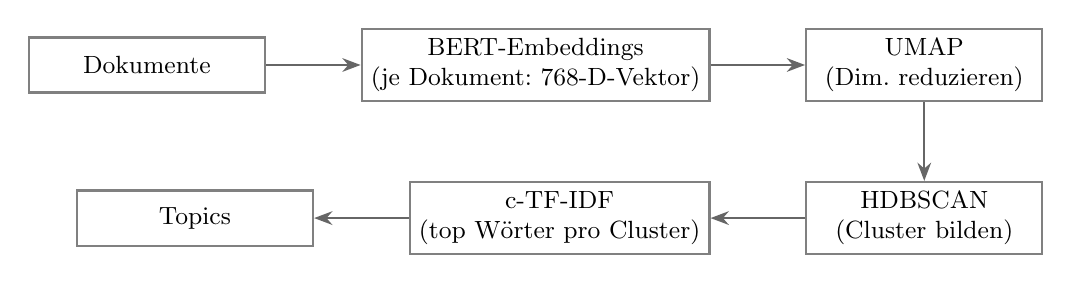
\begin{tikzpicture}[
        node distance=1.0cm,
        block/.style={rectangle,draw=black!50,thick,minimum width=3cm,minimum height=0.7cm,align=center,font=\small},
        arrow/.style={-Stealth,thick,black!60},
      ]
      \node[block] (a) {Dokumente};
      \node[block,right=1.2cm of a] (b) {BERT-Embeddings\\(je Dokument: 768-D-Vektor)};
      \node[block,right=1.2cm of b] (c) {UMAP\\(Dim.\ reduzieren)};
      \node[block,below=of c] (d) {HDBSCAN\\(Cluster bilden)};
      \node[block,left=1.2cm of d] (e) {c-TF-IDF\\(top Wörter pro Cluster)};
      \node[block,left=1.2cm of e] (f) {Topics};

      \draw[arrow] (a) -- (b);
      \draw[arrow] (b) -- (c);
      \draw[arrow] (c) -- (d);
      \draw[arrow] (d) -- (e);
      \draw[arrow] (e) -- (f);
    \end{tikzpicture}
  \end{center}

  \vfill
  Statt eine Matrix zu faktorisieren:
  \begin{enumerate}
    \item jeder Text wird zu einem \emph{Vektor} (BERT),
    \item Vektoren werden geclustert,
    \item für jeden Cluster wird die Wortliste durch eine angepasste
          TF-IDF-Heuristik berechnet (\emph{class-based TF-IDF}).
  \end{enumerate}

\end{frame}

% ===============================================================
\begin{frame}{BERTopic vs.\ LDA/NMF -- die Forschungslage}

  Empirische Vergleiche (Egger \& Yu 2022; Kaur \& Wallace 2024;
  Mishra 2026; Ma et al.\ 2025):

  \vfill
  \textbf{Wo BERTopic besser ist:}
  \begin{itemize}
    \item Bei \emph{kurzen} Texten (Tweets, SMS, Antworten auf
          offene Fragen).
    \item Bei semantisch \emph{nuancierten} Domänen, wo
          Ko-Okkurrenz allein nicht reicht.
    \item Höhere \emph{Topic-Kohärenz} in vielen Benchmarks.
  \end{itemize}

  \vfill
  \textbf{Wo LDA/NMF kompetitiv bleiben:}
  \begin{itemize}
    \item Bei \emph{längeren} Texten (Artikel, Interviews, Bücher).
    \item Wenn \emph{Interpretierbarkeit} und \emph{Reproduzierbarkeit}
          wichtiger sind als Kohärenz allein.
    \item Bei \emph{kleinen} Korpora -- BERTopic verlangt oft sehr
          viele Dokumente und verwirft 30--70\,\% als \emph{Outliers}
          (Soledad et al.\ 2022).
    \item Bei \emph{spezialisierten} Sprachen oder Disziplinen, für
          die kein guter vortrainierter BERT verfügbar ist.
  \end{itemize}

\end{frame}

% ===============================================================
\begin{frame}{Large Language Models in der Textanalyse}

  Seit 2022 verändert sich das Feld noch einmal. LLMs (GPT-4, Claude,
  LLaMA) können:

  \vfill
  \begin{itemize}
    \item Transkripte \textbf{zusammenfassen} und thematisch annotieren.
    \vfill
    \item Texte direkt \textbf{codieren} -- inklusive
          \emph{deduktiver} Codierung anhand eines Codebuches
          (Tai et al.\ 2024).
    \vfill
    \item \textbf{Themen erzeugen} oder \emph{labels} für vorhandene
          topics formulieren (TopicGPT, QualIT).
    \vfill
    \item \emph{Reflexive Co-Researcher} sein: Memos schreiben,
          Codierungswidersprüche aufzeigen (Sinha et al.\ 2024).
  \end{itemize}

  \vfill
  Eine umfangreiche Literatur ist seit 2023 entstanden: Bail (2023),
  Hayes (2025), Than et al.\ (2025), Tai et al.\ (2024).

\end{frame}

% ===============================================================
\begin{frame}{Aber: erste empirische Kritik}

  \begin{block}{Ashwin, Chhabra \& Rao (2025) -- \emph{Sociological Methods \& Research}}
    Untersuchung von Interviews mit Rohingya-Geflüchteten und
    bengalischen Gastgebern. Befund:

    \vspace{2pt}
    LLMs codieren \emph{systematisch verzerrt}: ihre Fehler sind
    \textbf{nicht zufällig} verteilt, sondern korrelieren mit den
    Merkmalen der Befragten (Sprache, Bildung, Region).
  \end{block}

  \vfill
  \textbf{Konsequenz:} Inferenzen, die auf LLM-Codierungen beruhen,
  können \emph{systematisch falsch} sein -- in eine \emph{bestimmte}
  Richtung.

  \vfill
  Die Autoren empfehlen: lieber ein \emph{eigenes, kleineres} Modell
  auf hochwertigen, manuell codierten Daten trainieren als einen
  generischen LLM einzusetzen.

  \vfill
  \footnotesize\color{black!60}
  Eine Erinnerung daran, dass auch \enquote{intelligente} Maschinen
  keine neutralen Werkzeuge sind.

\end{frame}

% ===============================================================
\begin{frame}{Warum bleibt MTA bei LDA und NMF?}

  Eine berechtigte Frage. Die Antwort hat \emph{vier} Aspekte:

  \vfill
  \begin{enumerate}
    \item \textbf{Lokal, offline, autonom.} MTA läuft auf Ihrem Laptop
          ohne Internetverbindung und ohne API-Schlüssel. Ihre Daten
          verlassen Ihre Maschine nicht.
    \vfill
    \item \textbf{Interpretierbarkeit.} LDA und NMF liefern \emph{nach\-voll\-zieh\-bare}
          Wortlisten und Gewichte. Sie können erklären, warum
          ein topic so aussieht, wie es aussieht.
    \vfill
    \item \textbf{Reproduzierbarkeit.} NMF mit festem Startwert
          produziert \emph{exakt dieselben} Ergebnisse. LLMs nicht.
    \vfill
    \item \textbf{Forschungsdidaktik.} Wer LDA/NMF versteht,
          versteht den \emph{Kern} der Topic-Modellierung. Wer mit
          BERTopic anfängt, ohne Embeddings zu kennen, arbeitet mit
          einer Blackbox.
  \end{enumerate}

\end{frame}

% ===============================================================
\section{Zwischenfazit}

\begin{frame}{Was wir heute gesehen haben}

  \begin{enumerate}
    \item Ein \textbf{topic} ist eine Gruppe von Wörtern, die oft
          gemeinsam vorkommen. Mathematisch: ein topic-Modell zerlegt
          die Dokument-Wort-Matrix in das Produkt zweier kleinerer
          Matrizen.
    \vfill
    \item Topic-Modelle unterscheiden sich von Clusteranalysen
          (\emph{mixed-membership}) und von Faktorenanalysen
          (\emph{nicht-negativ}, andere Verteilungsannahmen).
    \vfill
    \item \textbf{LDA} ist probabilistisch, \textbf{NMF}
          linearealgebraisch. Beide sind in MTA verfügbar und sollten
          \emph{verglichen} werden.
    \vfill
    \item \textbf{BERTopic} und \textbf{LLMs} sind die modernen
          Alternativen. Sie haben Stärken, aber auch ernsthafte
          methodologische Probleme. MTA bleibt aus guten Gründen bei
          LDA und NMF.
  \end{enumerate}

\end{frame}

% ===============================================================
\begin{frame}{Ausblick auf Sitzung 3}

  \textbf{Sitzung 3 -- Vom Verfahren zur Interpretation}

  \vfill
  \begin{itemize}
    \item Bevor der Algorithmus läuft: was ist ein \emph{Dokument}?
          Was sind \emph{Stoppwörter}? Wie reinigt man eine Textquelle?
    \vfill
    \item TF-IDF, Lemmatisierung, NER -- und was MTA \emph{nicht} tut.
    \vfill
    \item Metadaten und Topic-Modelle: drei Strategien.
    \vfill
    \item Der kritische Blick (Buch, Kap.~8): Was Topic-Modelle
          \emph{nicht} können. Zwei Erwartungen, die nicht erfüllt
          werden.
    \vfill
    \item Was sich für unsere Forschungspraxis ändert -- und wie
          diese drei Sitzungen in die folgende Arbeit mit MTA münden.
  \end{itemize}

\end{frame}

% ===============================================================
\begin{frame}[allowframebreaks]{Zitierte Literatur (Auswahl)}

  \footnotesize

  \textsc{Grundlage:} \\[2pt]
  Papilloud, C., \& Hinneburg, A.\ (2018). \emph{Einführung in die
  qualitative Analyse von Texten mit Topic-Modellen}. Wiesbaden:
  Springer. \emph{Bes.\ Kap.\ 2 und 3.}

  \medskip
  \textsc{Klassische Topic-Modelle:}
  \begin{itemize}
    \item Blei, D.\ M., Ng, A.\ Y., \& Jordan, M.\ I.\ (2003). Latent
          Dirichlet Allocation. \emph{Journal of Machine Learning
          Research}, 3, 993--1022.
    \item Lee, D.\ D., \& Seung, H.\ S.\ (2001). Algorithms for
          Non-Negative Matrix Factorization. \emph{NIPS}.
    \item Griffiths, T.\ L., \& Steyvers, M.\ (2004). Finding scientific
          topics. \emph{PNAS}, 101(suppl.\ 1), 5228--5235.
    \item Newman, D., Lau, J.\ H., Grieser, K., \& Baldwin, T.\ (2010).
          Automatic Evaluation of Topic Coherence. \emph{NAACL HLT}.
    \item Chang, J., et al.\ (2009). Reading Tea Leaves: How Humans
          Interpret Topic Models. \emph{NIPS}.
  \end{itemize}

  \medskip
  \textsc{Embeddings und BERT:}
  \begin{itemize}
    \item Mikolov, T., et al.\ (2013). Efficient Estimation of Word
          Representations in Vector Space. \emph{arXiv:1301.3781}.
    \item Devlin, J., et al.\ (2019). BERT: Pre-training of Deep
          Bidirectional Transformers. \emph{NAACL HLT}.
    \item Grootendorst, M.\ (2022). BERTopic: Neural Topic Modeling
          with a Class-based TF-IDF Procedure. \emph{arXiv:2203.05794}.
    \item Mostafavi, M., Porter, M.\ D., \& Robinson, D.\ T.\ (2025).
          Contextual Embeddings in Sociological Research.
          \emph{Sociological Methodology}.
  \end{itemize}

  \medskip
  \textsc{Empirische Vergleiche LDA/NMF/BERTopic:}
  \begin{itemize}
    \item Egger, R., \& Yu, J.\ (2022). A Topic Modeling Comparison
          Between LDA, NMF, Top2Vec, and BERTopic.
          \emph{Frontiers in Sociology}.
    \item Kaur, A., \& Wallace, J.\ R.\ (2024). Moving Beyond LDA:
          A Comparison of Unsupervised Topic Modelling Techniques.
          \emph{arXiv:2412.14486}.
    \item Mishra, M.\ (2026). Comparative Analysis of BERTopic Versus
          LDA: Topic Modelling in Marketing Research.
          \emph{Asia-Pacific Journal of Management Research}.
    \item Ma, L., et al.\ (2025). AI-powered topic modeling:
          comparing LDA and BERTopic.
          \emph{Experimental Biology and Medicine}.
  \end{itemize}

  \medskip
  \textsc{LLMs in der qualitativen Sozialforschung:}
  \begin{itemize}
    \item Hayes, A.\ S.\ (2025). \enquote{Conversing} With Qualitative
          Data: Enhancing Qualitative Research Through LLMs.
          \emph{International Journal of Qualitative Methods}.
    \item Ashwin, J., Chhabra, A., \& Rao, V.\ (2025). Using LLMs for
          Qualitative Analysis can Introduce Serious Bias.
          \emph{Sociological Methods \& Research}.
    \item Tai, R.\ H., et al.\ (2024). An Examination of the Use of
          Large Language Models to Aid Analysis of Textual Data.
          \emph{International Journal of Qualitative Methods}.
    \item Than, N., Fan, L., Law, T., Nelson, L.\ K., \& McCall, L.\
          (2025). Updating \enquote{The Future of Coding}: Qualitative
          Coding with Generative Large Language Models.
          \emph{Sociological Methods \& Research}.
    \item De Paoli, S.\ (2023). Performing an Inductive Thematic
          Analysis of Semi-Structured Interviews With a Large Language
          Model. \emph{Social Science Computer Review}.
  \end{itemize}

\end{frame}

% ===============================================================
\begin{frame}[plain]
  \begin{center}
    \vspace*{2em}
    {\Large\bfseries Vielen Dank.}
    \\[2em]
    Fragen, Einwände, Anschlüsse?
    \\[3em]
    \footnotesize\color{black!60}
    christian.papilloud@soziologie.uni-halle.de
  \end{center}
\end{frame}

\end{document}
